\documentclass{letnab}

\begin{document}
\begin{titlepage}
\center % Center everything on the page
 
%----------------------------------------------------------------------------------------
%	HEADING SECTIONS
%----------------------------------------------------------------------------------------

\textsc{\LARGE Московский Физико-Технический Институт}\\[1,5cm] % Name of your university/college
\textsc{\Large Кафедра общей физики}\\[0.5cm] % Major heading such as course name
\textsc{\large Лабораторная работа \textnumero  3.2.5}\\[0.5cm] % Minor heading such as course title

%----------------------------------------------------------------------------------------
%	TITLE SECTION
%----------------------------------------------------------------------------------------

\HRule
\\[0.4cm]
{ \huge \bfseries Вынужденные колебания в электрическом контуре}
\\[0.2cm] % Title of your document
\HRule
\\[1.5cm]


 
%----------------------------------------------------------------------------------------
%	AUTHOR SECTION
%----------------------------------------------------------------------------------------

\begin{minipage}{0.4\textwidth}
	\begin{flushleft} \large
		\emph{Автор:}\\
		Ришат \textsc{Исхаков} \\
		513 группа
	\end{flushleft}
\end{minipage}
~
\begin{minipage}{0.4\textwidth}
	\begin{flushright} \large
		\emph{Преподаватель:} \\
		Александр Александрович \textsc{Казимиров} % Supervisor's Name
	\end{flushright}
\end{minipage}

\begin{bottompar}
	\begin{center}
		
\includegraphics[width = 80 mm]{logo.jpg}
	\end{center}
	{\large \today}

\end{bottompar}
\vfill % Fill the rest of the page with whitespace

\end{titlepage}


\paragraph{Цель работы:} Исследование кривых намагничивания ферромагнетиков с помощью баллистического гальванометра.

\paragraph{В работе используются:} генератор тока с блоком питания, тороид, соленоид, баллистический гальванометр с осветителем и шкалой, амперметры, магазин сопротивлений, лабораторный автотрансформатор (ЛАТР), разделительный трансформатор.

\section{Теория}  

\begin{wrapfigure}[10]{r}{7cm}\vspace{-.9cm}
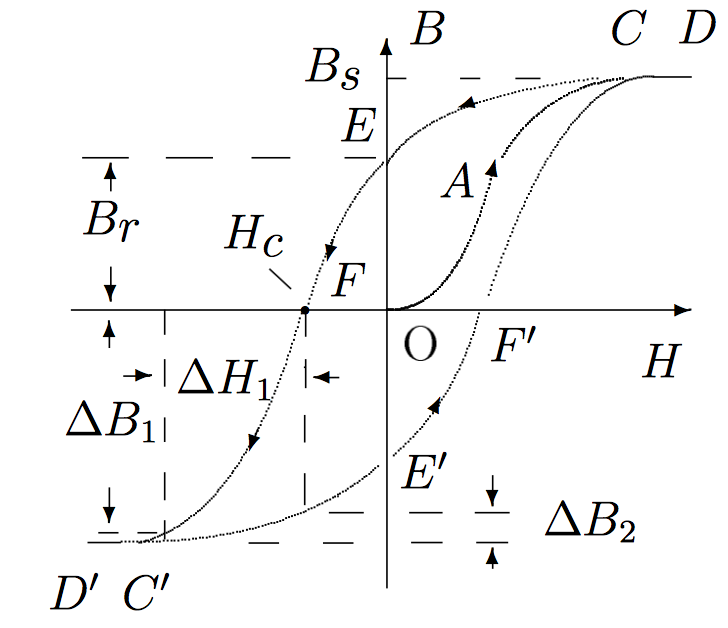
\includegraphics[width=.95\linewidth]{magnet}
\caption{Гистeрезис ферромагнетика}
\label{fig:magnet}
\end{wrapfigure} 

Магнитная индукция~$\mathbf{B}$ и напряженность магнитного поля~$\mathbf{H}$ в ферромагнетиках связаны между собой сложным нелинейным образом: индукция зависит не только от напряженности, но и от предыстории образца. Кривую намагничивания можно наблюдать на рис.~\ref{fig:magnet}. Выходящая из начала координат \textsf{основная кривая намагничивания} $OACD$ возникает при намагничивании размагниченного образца.

Зададимся целью определить коэрцитивную силу и индукцию насыщения предоставленного образца (материал~--- сталь).


\subsection{Предельная петля}

Индукция в образце складывается из напряжённости внешнего поля $\mathbf{H}$ и намагниченности образца: 
$\mathbf{B} = \mu_0 (\mathbf{H} + \mathbf{M})$, где \textsf{намагниченность} $\mathbf{M}$~--- магнитный момент единицы объема образца, а $\mu_0$~--- магнитная постоянная.

Сначала намагнитим образец до насыщения (точка $D$). Соответствующее значение индукции $B_s$ называют \textsf{индукцией насыщения}. Потом будем постепенно уменьшать внешнее поле. Явление гистерезиса состоит в том, что при нулевом значении внешнего поля индукция остаётся некоторая \textsf{остаточная индукция}~$B_r$. Чтобы размагнитить образец, то есть перевести его в состояние $F$, необходимо приложить «обратное» магнитное поле~$H_c$, которое называют \textsf{коэрцитивной силой}.

Замкнутая кривая $DEFD'E'F'D$, возникающая при циклическом перемагничивании образца, намагниченного до насыщения, называется \textsf{предельной петлей гистерезиса}.

\subsection{Формальное описание}

Необходимо выразить $H$ и $B$ через параметры, измеряемые в эксперименте. На тороидальный образец намотаны две обмотки~--- \textit{намагничивающая} с числом витков $N_{T0}$ и \textit{измерительная} с числом витков $N_{T1}$, подключенная к гальванометру, работающему в баллистическом режиме.

Напряженность магнитного поля в $H$ в тороиде зависит от тока, текущего в обмотке: 
$$H = \dfrac{N_{T0}}{\pi D} I,$$ где $D$~--- средний диаметр тора.

При скачкообразном изменении тока на величину $\Delta I$ поле в тороиде меняется: $\Delta H \sim \Delta I$. Изменение $\Delta H$ приводит к изменению потока магнитной индукции $\Phi$ в сердечнике, и в измерительной обмотке сечения $S_T$ с числом витков $\N_{T1}$ возникает ЭДС индукции:
$$\ef = - \dfrac{d \Phi}{dt} = - S_T N_{T1} \dfrac{dB}{dt}.$$

Через гальванометр протекает импульс тока; первый отброс зайчика гальванометра, работающего в баллистическом режиме, пропорционален величине прошедшего через гальванометр заряда $q$:
$$\varphi = \dfrac{q}{b},$$
где $b$~--- баллистическая постоянная гальванометра. 

Дополнительно для получения баллистической постоянной необходимо использовать вместо тороида пустотелый соленоид с числом витков $N_{T0}$, с $N_{T1}$ витками на измерительной катушке, длиной $l_c$. Тогда исключив баллистическую постоянную и выразив $\Delta B$ получим выражение:
$$\Delta B  = \mu_0 \left( \dfrac{d_C}{d_T} \right)^2 \dfrac{R}{R_1} \dfrac{N_{C0}}{N_{T1}} \dfrac{N_{C1}}{l_C} \Delta I_1 \dfrac{\Delta x}{\Delta x_1}.$$

\section{Описание установки}

\begin{figure}[H]
\centering
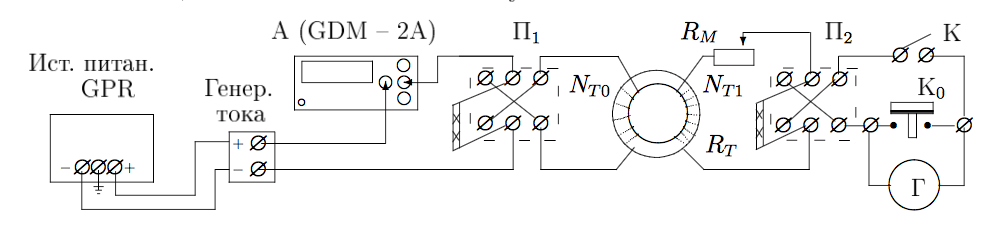
\includegraphics[width = 0.9 \tw]{scheme}
\caption{Схема экспериментальной установки для исследования петли гистерезиса}
\end{figure}

Измерение предельной петли гистерезиса начинаем с максимального значения магнитного поля, что соответствует точке $D$ на рис. \ref{fig:magnet}. Специальный генератор позволяет скачками менять токи в намагничивающей обмотке. Он работает неравномерно, так как разные скачки на разных участках петли вызывают разные отклонения зайчика гальванометра (большие скачки делаются вблизи насыщения и малые вблизи нуля). Дойдя до нулевого значения тока ($E$), меняем направление магнитного поля и снова увеличиваем ток в намагничивающей обмотке ($D'$). Затем снова меняем направление магнитного поля и возвращаемся в точку $D$.

Сопротивления измерительных цепей $R$ и $R_1$ подбираются одинаковыми, чтобы можно было считать постоянную гальванометра \emph{действительно} постоянной (она зависит от полного сопротивления в цепи).

Измерение начальной кривой намагничивания (участок $OAC$) производится по той же схеме, но с предварительно размагниченным образцом. 

\section{Измерения}

Измеренные значения $\Delta B$ откладываем по одной стороне петли от максимального значения индукции. Ось $H(I)$ проводится посередине петли. 

\begin{figure}[H]
\centering
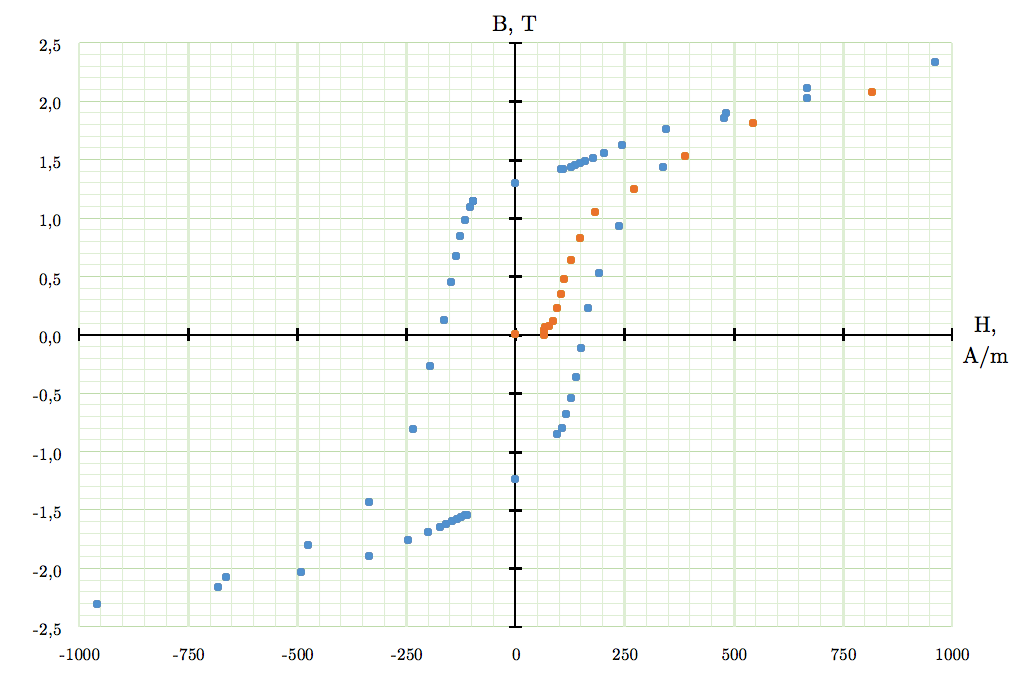
\includegraphics[width = .95\lw]{plot}
\caption{Полученная петля гистерезиса}
\end{figure}

Из графика получим значения коэрцитивную силу $H_c$ и индукцию насыщения $B_s$ и максимальное значение дифференциальной магнитной проницаемости $\mu_\text{диф}$:
$$H_c = 2.4 \pm 0.3 \text{ А/м}$$
$$B_s = 150 \pm 16 \; T$$
$$\mu_\text{диф} = \dfrac{1}{\mu_0} \dfrac{dB}{dH} = 6000 \pm 500$$
\begin{table}[H]
\centering
\begin{tabular}{|c|c|c|}
\hline 
 & Эксперимент & Теория \\ 
\hline 
$H_c, \text{ А/м}$ & $150 \pm 16$ & 140 \\ 
\hline 
$B_s, \; T$ & $2.4 \pm 0.3$ & 2.12 \\ 
\hline 
$\mu_\text{диф}$ & $6000 \pm 500$ & 4000 \\ 
\hline 
\end{tabular} 
\caption{Сравнение теории с практикой}
\end{table}
\section{Вывод}  

Было исследовано явление гистерезиса на примере образца стали (см. рис.~\ref{fig:magnet}). Она имеет две оси симметрии, выглядит вполне гладко и красиво, вписываясь в наше представление о природе вещей. Были оценены значения коэрцитивной силы $H_c$ и индукции насыщения $B_s$ и максимальное значение дифференциальной магнитной проницаемости $\mu_\text{диф}$. Значения с учетом погрешности совпадают с действительными.
\end{document}
